\documentclass[11pt,a4paper]{jsarticle}
%
\usepackage{amsmath,amssymb}
\usepackage{bm}
\usepackage[dvipdfmx]{graphicx}
\usepackage[dvipdfmx]{color}
\usepackage{ascmac}
\usepackage{listings}
%
\setlength{\textwidth}{\fullwidth}
\setlength{\textheight}{40\baselineskip}
\addtolength{\textheight}{\topskip}
\setlength{\voffset}{-0.2in}
\setlength{\topmargin}{0pt}
\setlength{\headheight}{0pt}
\setlength{\headsep}{0pt}
%
\newcommand{\divergence}{\mathrm{div}\,}  %ダイバージェンス
\newcommand{\grad}{\mathrm{grad}\,}  %グラディエント
\newcommand{\rot}{\mathrm{rot}\,}  %ローテーション
%
\title{レポート課題12}
\author{05-191009 奥村真司}
\date{}
\begin{document}
\maketitle
%
%
\section*{問1}
\subsection*{動作例}
\begin{lstlisting}[basicstyle=\ttfamily\footnotesize, frame=single]
?- ['problem1.pl'].
true.

?- eq(a,c).
ERROR: Out of local stack
\end{lstlisting}
\subsection*{考察}
仮定に以下のように番号をふることにする。
\begin{lstlisting}[basicstyle=\ttfamily\footnotesize, frame=single]
1. eq(a,b).
2. eq(c,b).
3. eq(X,Z) :- eq(X,Y),eq(Y,Z).
4. eq(X,Y) :- eq(Y,X).
\end{lstlisting}
各仮定の論理的な意味は以下のようになる。
\begin{itemize}
	\item $1. eq(a,b)$
	\item $2. eq(c,b)$
	\item $3. \forall X \forall Y \forall Z. eq(X,Y) \land eq(Y,Z) \rightarrow eq(X,Z)$
	\item $4. \forall X \forall Y eq(Y,X) \rightarrow eq(X,Y)$
\end{itemize}
仮定2より$eq(c,b)$,これと仮定4で$X=c,Y=b$としたものから、$eq(b,c)$。仮定1よりeq(a,b)であるから$eq(a,b)\land eq(b,c)$。これと仮定3で$X=a,Y=b,Z=c$としたものより$eq(a,c)$よって$eq(a,c)$はtrueである。\par
Prologは番号の若いルールを優先して深さ優先探索によってSLD導出を探索する。よって探索は以下の画像のように進み、無限ループし、処理系に実際に問い合わせるとスタックオーバーフローした。論理的解釈と一致させるには、処理系の探索方法を幅優先探索にすればよい。実際発展2の処理系ではtrue.が表示される。
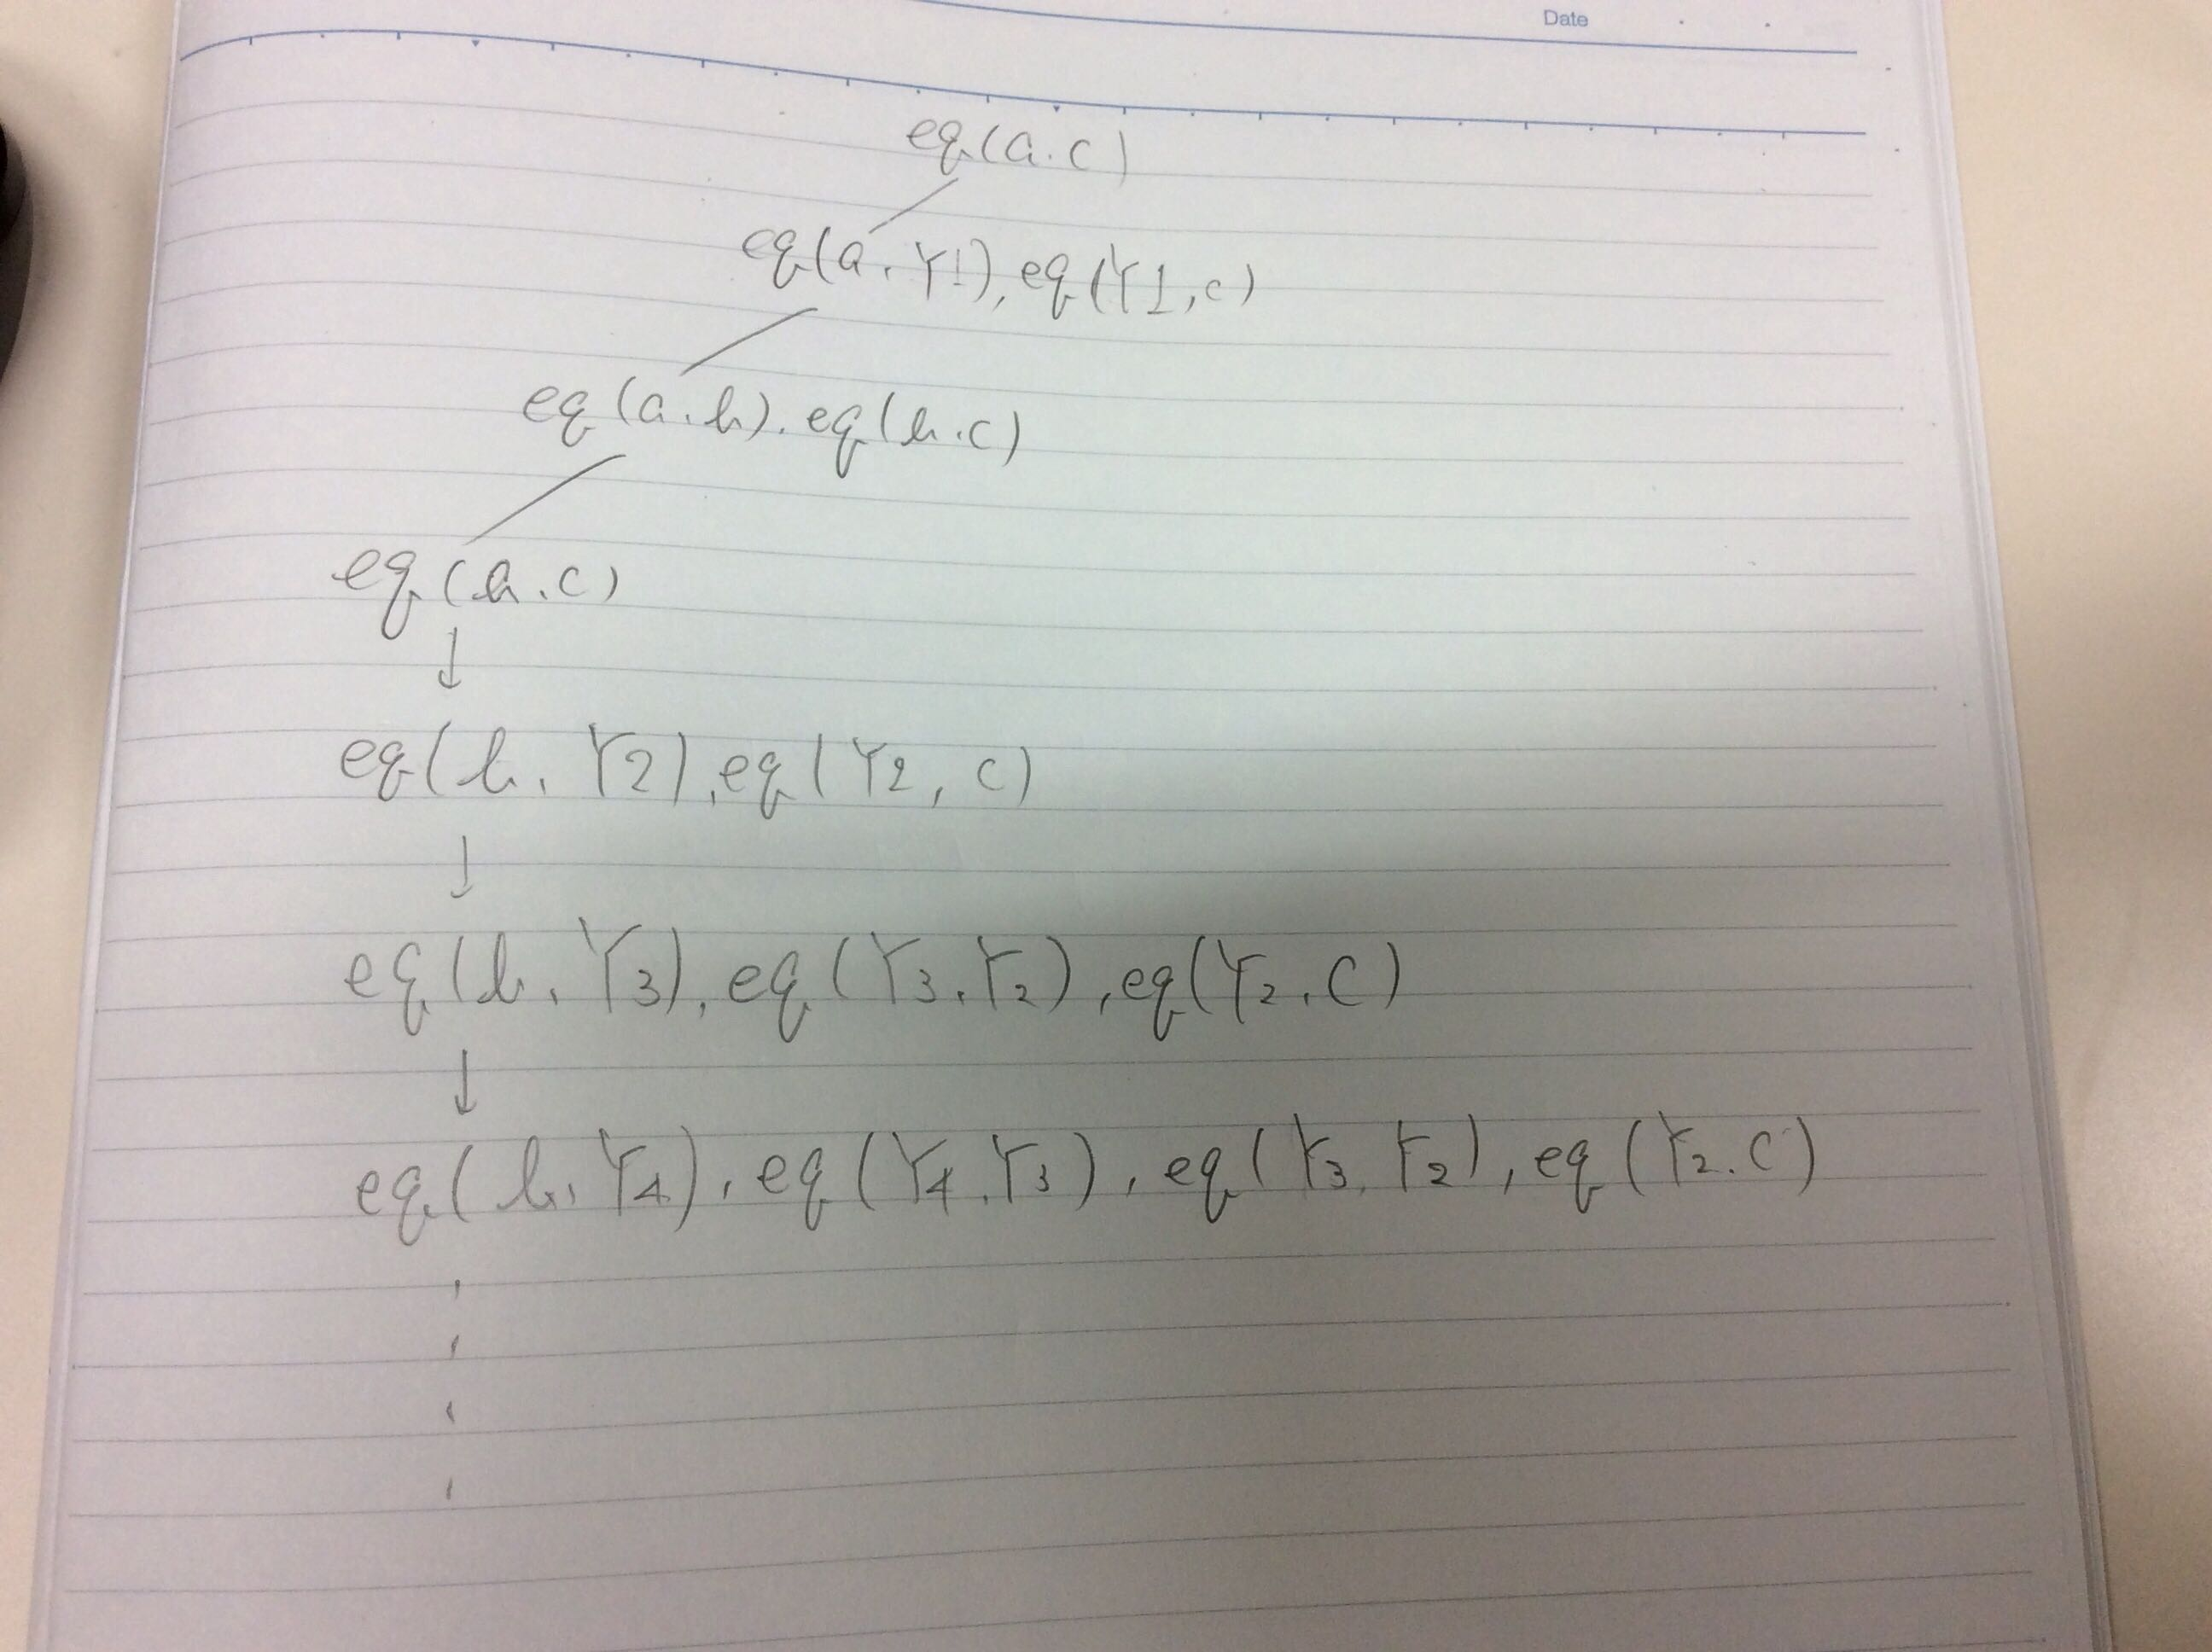
\includegraphics[width=14.5cm]{problem1.jpg}\par
\section*{問2}
\begin{lstlisting}[basicstyle=\ttfamily\footnotesize, frame=single]
?- ['problem2.pl'].
true.

?- test.
true.

?- q(X,X).
X = f(X).
\end{lstlisting}
\subsection*{考察}
論理的解釈では、q(X,X)とq(X,f(X))は単一化できないので、falseとなると考えられる。しかし動作例のようにtest.をProlog処理系に問い合わせるとtrueとなる。これは、Prolog処理系が単一化の際に出現検査をしていないからであり、q(X,X)を問い合わせると動作例のようにX=f(X)と出力される。この出現検査の有無が論理的解釈との差異を生んでいる。
\section*{問3}
\begin{lstlisting}[basicstyle=\ttfamily\footnotesize, frame=single]
?- ['problem3.pl'].
true.

?- \+p(X),q(X).
false.

?- q(X),\+p(X).
X = b.
\end{lstlisting}
\subsection*{考察}
閉世界仮説より、
$\forall X.(p(X) \leftrightarrow X=a)$,$\forall X.(q(X)\leftrightarrow X=b)$であるから、$\lnot p(b)$はtrueで$q(b)$もtrue,すなわち$\lnot p(b) \land q(b)$がtrueなので$\exists X.(\lnot p(X) \land q(X))$は論理的解釈ではtrueと考えられる。\par
Prolog処理系で実際に問い合わせると、動作例のようにfalseが帰ってくる。Prolog処理系での否定は導出の失敗による否定で、変数が含まれる場合にもこれが適用される。処理系に問い合わせると、p(X)が導出できるかどうかを探索するが,p(a)がtrueで導出できるのでY\llap=+p(X)はfalseとなる。よってY\llap=+p(X),q(X)もfalseとなる。このように、Prolog処理系は内部に変数を含む項にたいしても失敗による否定を適用することが論理的解釈との差異を生んでいる。\par
論理的解釈と結果を一致させるためにはPrologがゴールを解決しようとするときにそれに含まれる変数がすべて変数を含まないものに置き換わっているようにすればよいので、問い合わせをq(X),Y\llap=+p(X).に書き換えると、動作例のようにtrue.となる。この場合は探索中にXはbに置き換わり、ゴールの導出に成功する。\\

\section*{発展1}
\subsection*{動作例}
\begin{lstlisting}[basicstyle=\ttfamily\footnotesize, frame=single]
?- ['advanced1.pl'].
true.

?- r(a).
ERROR: Out of global stack
\end{lstlisting}
\subsection*{考察}
論理的解釈では、p(a)はtrueもしくはfalseのどちらかである。p(a)がtrueの場合は仮定1より、falseの場合は仮定2より、いずれの場合もr(a)はtrueとなるので,r(a)がtrueは論理的帰結である。\par
r(a).を問い合わせると、処理系はルール1よりp(a)の導出を試みる。しかしゴールは$p(a)\rightarrow p(f(a)) \rightarrow p(f(f(a))) \rightarrow p(f(f(f(a)))) \rightarrow ...$となり無限ループする。
Prologの否定は失敗による否定で、p(a)の導出に成功すればY\llap=+p(a)の導出は失敗し、p(a)の導出に失敗すればY\llap=+p(a)の導出は成功する。しかしp(a)の導出が成功も失敗もせず無限ループした場合、Y\llap=+p(a)の導出は成功も失敗もしないが、p(a)の導出が無限ループする場合、論理的解釈においては$p(a)$がfalse,$\lnot p(a)$がtrueである。(ただし変数を含まない時)
\section*{発展2}
\subsection*{動作例}
\begin{lstlisting}[basicstyle=\ttfamily\footnotesize, frame=single]
?- rule eq(a,b).
?- rule eq(c,b).
?- rule eq(X,Z) :- eq(X,Y),eq(Y,Z).
?- rule eq(X,Y) :- eq(Y,X).
?- query eq(a,c).
true.
----------------------------------------
?- rule test :- q(X,X).
?- rule q(X,f(X)).
?- query test.
false.
\end{lstlisting}
\subsection*{考察}
基本的には前回の課題の発展1のインタプリタである。否定は実装していない。(採点の担当の方が先週と違う場合を考えてこのレポートの最後の部分に前回の発展1のレポートを引用しております。適宜参照していただけるとありがたいです。)
以下で論理的に健全で完全であることを説明する。
Prolog処理系とことなり深さ優先探索ではなく幅優先探索をしているので、証明(木)は有限の深さであるから証明が存在するならば、今回実装した処理系は必ず有限時間でそれを発見し報告できる。幅優先探索にすることで自然にルールの優先順位が取り払われている。ここでここまでの方法とSLD導出の定義のスライドと見比べたときに異なる点は"ゴールリストのサブゴールを1つ選ぶ"という点で、先週の処理系ではかならずゴールリストの先頭を選ぶようになっていたのでここが任意に一つ選ばれるように改良した。
今回の問2で見たように、単一化の際の出現検査をしないと論理的解釈と差異が生じるので、単一化の出現検査をちゃんとやるようにしている。よってSLD導出の健全性、完全性より今回実装したPrologライクな論理型言語は完全かつ健全ある。\par
動作例では,問1,問2でPrologでは論理的解釈と差異が生じていたものが、今回実装したものでは差異を生じないことが確認できる。
\newpage
\hrulefill
\section*{前回の発展1(前回分レポートより引用)}
\subsection*{動作例}
\begin{lstlisting}[basicstyle=\ttfamily\footnotesize, frame=single]
?- rule nat(z).
?- rule nat(s(X)) :- nat(X).
?- query nat(X).
X = z
;
X = s(z)
;
X = s(s(z))
;
X = s(s(s(z)))
;
X = s(s(s(s(z))))
;
X = s(s(s(s(s(z)))))
;
X = s(s(s(s(s(s(z))))))
;
X = s(s(s(s(s(s(s(z)))))))
.
?- rule male(koji).
?- rule parent(kobo,koji).
?- rule father(X,Y) :- parent(X,Y),male(Y).
?- query father(kobo,Z).
Z = koji
;
false.
?- rule add(z,Y,Y).
?- rule add(s(X),Y,s(Z)) :- add(X,Y,Z).
?- query add(s(z),X,X).
false.
?- rule append([],Y,Y).
?- rule append([A|X],Y,[A|Z]) :- append(X,Y,Z).
?- rule concat([X|[]],X).
?- rule concat([X|Y],Z) :- concat(Y,W),append(X,W,Z).
?- query append([1,2,3],[4,5],Z).
Z = [1, 2, 3, 4, 5]
;
false.
?- query append(X,Y,[1,2,3,4,5]).
Y = [1, 2, 3, 4, 5]
X = []
;
Y = [2, 3, 4, 5]
X = [1]
;
Y = [3, 4, 5]
X = [1, 2]
;
Y = [4, 5]
X = [1, 2, 3]
;
Y = [5]
X = [1, 2, 3, 4]
;
Y = []
X = [1, 2, 3, 4, 5]
;
false.
?- query concat([[1],[2,3,4]] ,X).
X = [1, 2, 3, 4]
;
false.
?- rule in(X,[X|Y]).
?- rule in(X,[Y|Z]) :- in(X,Z).
?- rule choose([X|Y],Y,X).
?- rule choose([A|X],[A|Y],Z) :- choose(X,Y,Z).
?- rule hamilton(V,E) :- choose(V,Rem,Start),hamiltonsub(Rem,E,Start).
?- rule hamiltonsub([],X,Y).
?- rule hamiltonsub(V,E,Now) :- choose(V,Rem,Next),in([Now|[Next|[]]],E),
hamiltonsub(Rem,E,Next).
?- query hamilton([1,2,3,4],[[1,2],[2,3],[3,4],[4,1]]).
true.
;
true.
;
true.
;
true.
;
false.
?- query abcd.
Undefined procedure.
?- query a([,
Parse Error.
?- $
Failure Unknown Token: $
\end{lstlisting}
\subsection*{考察}
Prologライクな論理型言語のインタプリタをレクサー、パーサーも含め実装した。動作例のように、前回の授業で扱ったものや課題の解答で自分で作成したものについて、期待通りに動作することがわかった。addの例では出現検査をちゃんと行えていることが確認できた。この動作例における入力データはverify.pl内にある。
\subsubsection*{定数、項、述語などの扱い}
実装を始めるにあたってまず定数、項、述語などのデータをどう扱うかを考えた。これらの文法はPrologと同じようにした。syntax.ml内でこれらの型は下のように定義されている。
\begin{lstlisting}[basicstyle=\ttfamily\footnotesize, frame=single]
type name = string 
type var = int

type term =
  | EConst of name
  | EFnSymb  of name * (term list)
  | EVar of name
  | ECons of term * term
  | ENil

type fact = EPdSymb of name * (term list)

type rule = fact * (fact list)

type command =
  | CRule    of rule
  | CQuery   of fact list
  | CCont
  | CExit

type subst = (name * term) list

type constraints = (term * term) list
\end{lstlisting}
termが授業スライドでの項にあたるもので、定数がEConst,ファンクタがEFnSymb(Function Symbol),..というようになっている。述語(項,項,...)をfactという名前にした(この形式にfactという名前をつけただけでこれが意味的にfactとは限らない。例えば問い合わせでのゴールのリストはfact listである。)。述語(項,項,...) :- 述語(項,項,...),述語(項,項,...),...がruleである。\par
ルールの読み込みと問い合わせの区別は入力の先頭にruleかqueryとつけることを要求することで実現した。queryではそこまでに入力されたrule全てを用いてSLD導出を探索する。
\subsubsection*{探索}
次に探索について説明する。授業スライドにもあるとおりSLD導出を探索しているが、swi-prologと異なり幅優先探索(BFS)で探索し、単一化時に出現検査を行うようにした。\par
ゴールのリストの先頭とルールを単一化する際に、入力された通りの変数名を用いると変数名がかぶっているときに正しく単一化できないので、ルールを用いるたびに内部の変数名をすべてuniqueなものに置き換えている。がsyntax.ml内のconvert\_$****$という関数群はこの置き換えを行うための補助関数である。
例えば$\texttt{father(X,Y) :- parent(X,Y),male(Y)}$というruleなら、$\texttt{father(\_1,\_2) :- parent(\_1,\_2),male(\_2)}$のように置き換えられる。同じルールでも置き換えを行うたびに別のものになる。\par
探索の各状態はfact list型のゴールのリストとsubst型の置き換えの組になっている。
BFSの実現方法について説明する。BFSはQueueを用いて行った。計算量的には好ましくないが、listをqueueとみなし@で後ろにつなげることでpushを、先頭の取り出しはパターンマッチで行っている。eval内のnextという関数は探索状態と仕様するルールを受け取って、ゴールリストの先頭とルールが単一化可能なら次の状態のsigletonリストを,不可能なら空リストを返す関数であり、$\texttt{List.concat (List.map (fun r -> next q r) rules)}$とすることで現在の状態qからルールrulesを用いて遷移可能な状態のリストが得られる。これをqueueの後ろに@でつないでいる。これを@で前につなぐように変更するだけで簡単にDFSにすることもできる。解が見つかったらその時点でのqueueの状態も一緒に返してやることで、続きからの探索も可能になっている。
\subsubsection*{その他こだわりポイント}
以下は課題の出題意図とは直接的には関係ないと思われるがこだわった点について説明する。
\begin{itemize}
	\item リストの[x,y,z]の入出力形式のサポート\par
	はじめはコンスの形のみサポートしていたが非常に入力しづらいので[x,y,z]の形式をサポートした。これが意外と思考を要したのでそれについて説明する。$\texttt{[a|b]}$を以下の画像のように捉えることで、termの構造はEConsによる完全二分木と捉えることができる。[x,y,z],[x,y,z$|$w]は下のような木構造を表すことから、[x,y,z]は[x,y,z$|$[]]の省略形と思える。
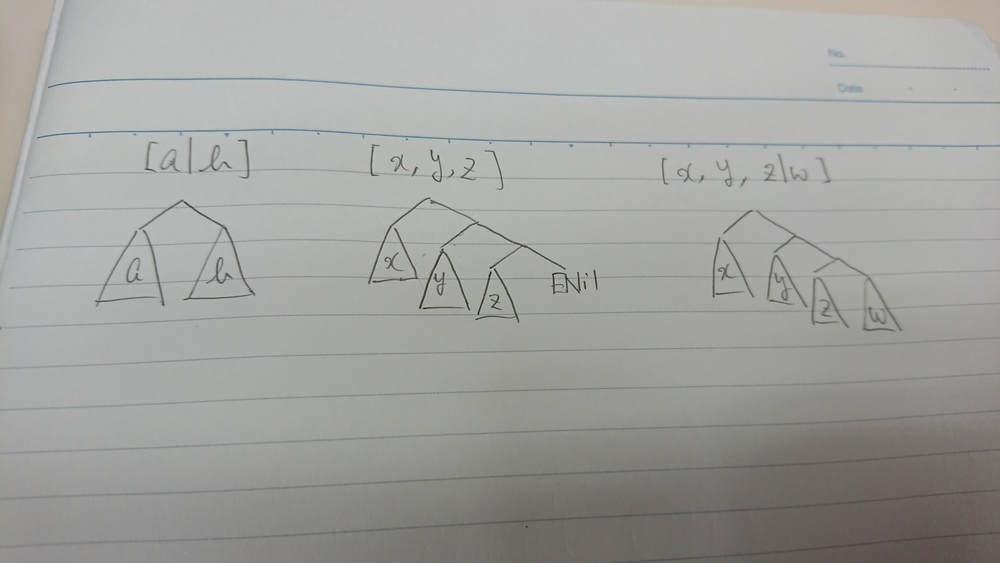
\includegraphics[width=14.5cm]{LsitTree.jpg}\par
	よって、最後の要素で場合分けして考えることでParserは以下のように書けた。
\begin{lstlisting}[basicstyle=\ttfamily\footnotesize, frame=single]
atomic:
  | SYMBID { EConst($1) }
  | NUMBER { EConst($1) }
  | VARID  { EVar($1) }
  | list   { $1 }
;

atomics:
  | list_last { $1 }
  | atomic COMMA atomics { ECons($1,$3) } 
;

list_last:
  | atomic { ECons($1,ENil) }
  | atomic BAR atomic { ECons($1,$3) }
;

list:
  | NIL { ENil }
  | LBRACKET atomics RBRACKET { $2 }
;
\end{lstlisting}
出力も、カンマを出力すべきかどうかをパターンマッチで場合わけして以下のように書くことができた。
\begin{lstlisting}[basicstyle=\ttfamily\footnotesize, frame=single]
let rec print_term t = 
  match t with
  | EFnSymb (id,tl) -> print_name id;
                       if tl=[] then ()
                                else (print_string "(";
                                      print_term_list tl;
                                      print_string ")")
  | EVar id -> print_name id
  | ECons (x,y) -> print_list t
  | ENil -> print_string "[]"
  | EConst x -> print_name x 
and print_term_list tl = 
  match tl with
  | [] -> ()
  | t::rest -> print_term t;
               (if (rest <> []) then (print_string ",") 
                                else ());
               print_term_list rest
and print_list t =
  print_string "[";
  print_list_inner t;
  print_string "]"
and print_list_inner t =
  match t with
  | ECons (x,(ECons(y,z))) -> print_term x;
  		   	  print_string ", ";
  		   	  print_list_inner (ECons (y,z))
  | ECons (x,ENil) -> print_term x
  | ECons (x,y) -> print_term x;
  		   print_string " | ";
  		   print_term y
  | _ -> () (* Error *)
\end{lstlisting}
	\item エラー\par
	動作例の最後から3つめのように、全く定義されていない述語についての問い合わせが来た場合に、閉世界仮説的にはfalse.でいいのではないかと思ったが、swi-prologではUndefined procedureというエラーが出るようになっていたのでそれを採用し、チェックするようにした。
	動作例の最後のあたりのように、レクサーやパーサーのエラーも含めエラーが発生しても処理系はエラーメッセージを出力して次の入力を待ち、終了しないようにした。なおエラー出力およびfalse.はbashで赤文字で出力されるようにした。
\end{itemize}
\end{document}
